% Important: If latex complains about unicode characters,
% please use "\usepackage[utf8x]{inputenc}" in your preamble
% You can change the size of the picture by putting it into the construct:
% 1) \resizebox{10cm}{!}{"below picture"} to scale horizontally to 10 cm
% 2) \resizebox{!}{15cm}{"below picture"} to scale vertically to 15 cm
% 3) \resizebox{10cm}{15cm}{"below picture"} a combination of above two
% It is not recomended to use the scale option of the tikzpicture environment.
\resizebox{7cm}{!}{
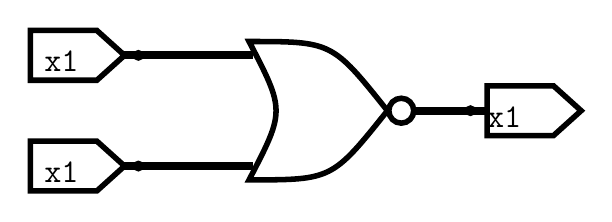
\begin{tikzpicture}[x=1pt,y=-1pt,line cap=rect]
\def\logisimfontA#1{\fontfamily{cmr}{#1}} % Replaced by logisim, original font was "SansSerif"
\def\logisimfontB#1{\fontfamily{cmtt}{#1}} % Replaced by logisim, original font was "Monospaced"
\definecolor{custcol_0_0_0}{RGB}{0, 0, 0}
\definecolor{custcol_ff_ff_ff}{RGB}{255, 255, 255}
\draw [line width=3.0pt, custcol_0_0_0 ]  (145.0,35.0) -- (165.0,35.0) ;
\draw [line width=2.0pt, custcol_0_0_0 ]  (135.0,35.0) .. controls  (115.0,10.0)  ..  (85.0,10.0) .. controls  (98.0,35.0)  ..  (85.0,60.0) .. controls  (115.0,60.0)  ..  (135.0,35.0) -- cycle ;
\draw [line width=2.0pt, custcol_0_0_0]  (140.0,35.0) ellipse (4.5 and 4.5 );
\draw [line width=3.0pt, custcol_0_0_0 ]  (40.0,55.0) -- (45.0,55.0) -- (85.0,55.0) -- (85.0,55.0) ;
\draw [line width=2.0pt, custcol_0_0_0 ]  (30.0,64.0) -- (40.0,55.0) -- (30.0,46.0) -- (6.0,46.0) -- (6.0,64.0) -- cycle;
\logisimfontB{\fontsize{12pt}{12pt}\selectfont\node[inner sep=0, outer sep=0, custcol_0_0_0, anchor=base west] at  (11.0,61.0)  {x1};}
\fill [line width=2.0pt, custcol_0_0_0]  (45.0,55.0) ellipse (2.0 and 2.0 );
\draw [line width=3.0pt, custcol_0_0_0 ]  (40.0,15.0) -- (45.0,15.0) -- (85.0,15.0) -- (85.0,15.0) ;
\draw [line width=2.0pt, custcol_0_0_0 ]  (30.0,24.0) -- (40.0,15.0) -- (30.0,6.0) -- (6.0,6.0) -- (6.0,24.0) -- cycle;
\logisimfontB{\fontsize{12pt}{12pt}\selectfont\node[inner sep=0, outer sep=0, custcol_0_0_0, anchor=base west] at  (11.0,21.0)  {x1};}
\fill [line width=2.0pt, custcol_0_0_0]  (45.0,15.0) ellipse (2.0 and 2.0 );
\draw [line width=3.0pt, custcol_0_0_0 ]  (169.0,35.0) -- (166.0,35.0) ;
\draw [line width=2.0pt, custcol_0_0_0 ]  (195.0,26.0) -- (205.0,35.0) -- (195.0,44.0) -- (171.0,44.0) -- (171.0,26.0) -- cycle;
\logisimfontB{\fontsize{12pt}{12pt}\selectfont\node[inner sep=0, outer sep=0, custcol_0_0_0, anchor=base west] at  (171.0,41.0)  {x1};}
\fill [line width=2.0pt, custcol_0_0_0]  (165.0,35.0) ellipse (2.0 and 2.0 );
\end{tikzpicture}
}
